The SSP1-MOB vision of the future described in \sref{s:results:ssp1-mob} is used in the following sections to synthesise the changes that the mobility paradigm must undergo\footnote{The changes are not ``suffered'' by an autonomous and disconnected system of mobility, but are introduced by all the agents that play a part in it: users, industries, governments, decision makers, researchers, planners, etc.} to reach the desired form. The synthesis is done using backcasting approach, for which an ``intermediate step'' is presented in \ssref{ss:results:backcasting-2050-intermediate-step}. This halfway step is described in terms of the same variables highlighted in \tref{t:ssp1-mob-2100-narrative-thesis}, but adding information for the year 2050. The baseline ``scenario'' status of 2017 is also provided in \ssref{ss:results:backcasting-2050-intermediate-step}. The changes between the 2100 and 2050 storylines, along with the ones between the 2050 narrative and the baseline are then provided in \ssref{ss:results:backcasting-the-path}.

\subsection{SSP1-MOB 2050: an intermediate step to sustainable mobility}
\label{ss:results:backcasting-2050-intermediate-step}
In order to ease the identification of changes and trends within the backcasting process of \ssref{ss:results:backcasting-the-path}, an intermediate step for the year 2050 is developed and displayed in \tref{t:ssp1-mob-2050-narrative-thesis}. The comparison table contains the variables for the 2100, 2050 and 2017 (baseline) years. With regards to the baseline, numerous data sources have been consulted, with as high as possible quality standards. The list of sources mainly consists of databases from global agencies or multinational regions, like the International Energy Agency (IEA) or the European Commission (EC). \todonote{Should this be in the Methods chapter?}Even though there are some inconsistencies regarding the data collection years, the range is considerably limited: only data from 2005 is considered. However thorough the baseline data research was, some variables were actually assumed to have some (qualitative) value, which is generally aligned with the insights that authors dealing with sustainable mobility provide. \todonote{Is the following true for \textbf{all} variables??}For all those variables where an estimation was infeasible or supporting data was unavailable, an ``assumed'' label is displayed.
%

% backcasting table 2017 2050 2100 states
\begin{landscape}
{\tiny
\begin{longtable}{p{3cm}p{5cm}p{5cm}p{5cm}}
\caption[Comparison of SSP1-MOB qualitative variables (2017, 2050 and 2100)]{Comparison of SSP1-MOB qualitative variables (2017, 2050 and 2100).}\\
\toprule
& \multicolumn{3}{l}{Trend or status}\\	
\cmidrule(l){2-4} Variable or feature & 2017 & 2050 & 2100\\
\midrule
\endfirsthead
\caption*{(\emph{continued}) Comparison of SSP1-MOB qualitative variables (2017, 2050 and 2100)}\\
\toprule
& \multicolumn{3}{l}{Trend or status}\\
\cmidrule(l){2-4} Variable or feature & 2017 & 2050 & 2100\\
\midrule
\endhead
\bottomrule
\endfoot
\bottomrule \addlinespace
\multicolumn{4}{l}{\textsuperscript{1}Tpkm/yr stands for ``tera passenger-kilometers per year''}\\
\multicolumn{4}{l}{\textsuperscript{2}M stands for millions (population)}\\
\multicolumn{4}{p{14cm}}{\textsuperscript{3}Only 12\% of the total 993 reported fatalities linked to rail in the EU were passengers or employees. The remaining 88\% were people at, e.g., level-crossings or unauthorised people at rail premises \parencite{eurostat2017_StatisticsExplainedRailway}}\\
\multicolumn{4}{l}{\textsuperscript{4}WECs: Western European Countries; CEECs: Central and Eastern European Countries}\\
\multicolumn{4}{l}{\textsuperscript{5}HICs: High Income Countries; LICs: Low Income Countries (considered in terms of the baseline situation)}\\
\endlastfoot
\label{t:ssp1-mob-2050-narrative-thesis}\textbf{Development scenario} &  &  &  \\*
Societal sustainability awareness & Low (assumed) & Medium & High \\*
Total travel demand (Tpkm/yr) & approx. 50 Tpkm/yr\textsuperscript{1} in 2010 \parencite{vuuren2017_Energylanduse} & Higher than the baseline (2017) & Higher than the baseline (2017) \\*
Travel demand per capita (Tpkm/yr) & approx. 7300 pkm/yr in 2010 \parencite{vuuren2017_Energylanduse,kc2017_humancoreshared} & Similar to the baseline (2017) & Lower than the baseline (2017) \\\addlinespace
\textbf{Land use (urban development)} &  &  &  \\*
Urban density & 0.9\% urban pop. in \textgreater40000 p/km2 areas; 4.8\% in 20000-40000 p/km2; 18.3\% in 10000-20000 p/km2, 51.4\% in 4000-10000 p/km2; 15.2\% in 2000-4000 p/km2 and 9.4\% in \textless2000 p/km2 \parencite{cox2017_DemographiaWorldUrban} & Medium-high and increasing & High (higher than 2017 baseline) \\*
Urban use patterns & Single-use is widespread, mixed-use for cities & Mixed-use development paradigm & Mixed-use development paradigm \\*
Economic centralisation & High; metropolis accumulate a big share of the activity & High; metropolis accumulate a big share of the activity & Medium; cities are hotspots, but jobs are spread amongst them \\*
City sizes & 8.4\% \textgreater10M\textsuperscript{2}, 4.2\% 5-10M, 5.4\% 2.5-5M, 6.5\% 1-2.5M, 4.8\% 0.5-1M, 70.7\% \textless0.5M \parencite{cox2017_DemographiaWorldUrban} & Medium to large; megacities and (sub)urban sprawl beginning to shrink & Medium; avoidance of megacities or (sub)urban sprawl \\\addlinespace
\textbf{Travel modes share} &  &  &  \\*
Intermodal travel & Long distance (\textgreater100 km) travel is mostly (80\%) by car. Intermodality is confined to urban and regional mobility. \parencite{riley2010_IntermodalPassengerTransport} & Facilitated, but still not common & Facilitated, high acceptancy and usage \\*
Public transport (rail, bus, aviation) & 40.17\% share (pkm/yr) approx. from \parencite{vuuren2017_Energylanduse} & Increasing demand supply; higher than the baseline (2017) & Majority of demand supply; much higher than the baseline (2017) \\*
Automobility (private vehicles) & 35.90\% share (pkm/yr) approx. from \parencite{vuuren2017_Energylanduse} & Lower than the baseline (2017) & Still relevant, but much lower than the baseline (2017) \\*
Slow modes (walking and cycling) & 23.93\% share (pkm/yr) approx. from \parencite{vuuren2017_Energylanduse} & Moderate increase compared to baseline (2017) & Higher than the baseline (2017) \\\addlinespace
\textbf{Cultural perception} &  &  &  \\*
Mobility & Understood as a right and an individual-social emancipation mechanism (through tourism and recreational mobility) \parencite{sheller2008_MobilityFreedomPublic} & Accessibility as a focus, managed, reasonable travel time, integrated & Accessibility, local in scale, slowed down, managed, reasonable travel time and reliability, integrated \\*
Public transport & PT as an affordable solution, but marginal and regarded as a low-status form of mobility & Public mobility as an affordable and accessible service & Public mobility as a reliable, comfortable, enjoyable and accessible service \\*
Automobility & Shaped by structured stories of ``joy of driving'', freedom and individuality discourses \parencite{gartman2004_ThreeAgesAutomobile,sheller2012_EmergenceNewCultures} & Automobility fills accessibility gaps; symbolic status decreasing & Automobility as a utility to serve a special need \\\addlinespace
\textbf{Public transport} &  &  &  \\*
Consumer cost & Medium-High (in many countries, public transport is not affordable for the 20\% lowest-in-income population \parencite{carruthers2005_AffordabilityPublicTransport}) & Low & Low \\*
Accessibility & Low (assumed) & Medium-high & High \\*
Safety & Fatalities (EU): 993 railway (27 passengers, 34 employees, 932 other\textsuperscript{3}), 155 aviation, (2015) \parencite{eurostat2017_EurostatOnlineDatabase} & High & High \\*
Public transport infrastructure investments & Rail: approx. 30\% of total infrastructure investments in Europe (2010, average for WECs\textsuperscript{4} and CEECs\textsuperscript{4}) \parencite{kauppila2012_OECDCountriesSpend} & High and continuous & High and continuous \\\addlinespace
\textbf{Automobility} &  &  &  \\*
Consumer cost & Low-Medium (assumed) & Medium & High \\*
Accessibility & High (assumed) & High & High (especially in rural or remote areas) \\*
Safety & 1.2M road deaths in the world, 28077 in the EU (2013) \parencite{who2017_GlobalHealthObservatory} & Medium (especially Low Income Countries) & High (higher risk than public transport) \\*
Automobility infrastructure investments & Roads: approx. 70\% of total infrastructure investments in Europe (2010, average for WECs and CEECs) \parencite{kauppila2012_OECDCountriesSpend} & Medium; maintenance dominates in HICs\textsuperscript{5}; capacity increased in LICs\textsuperscript{5} & Low to medium; maintenance covers the majority of the investments; capacity is not increased \\\addlinespace
\textbf{Fuel technology} &  &  &  \\*
Automobiles & 96\% fossil fuels (oil products \& natural gas), 4\% biofuels \parencite{iea2017_Statisticswebportal} & Battery electric vehicles and hybrids for short-medium ranged trips; biofuelled for long range & Battery electric vehicles for short-medium ranged trips; hydrogen fuelled for long range \\*
Rail & 57.3\% oil, 5.6\% coal, 36.4\% electricity \parencite{cazzola2016_RailwayHandbook2016} & Full electrification of the network & Full electrification of the network \\*
Bus & 96\% fossil fuels (oil products \& natural gas), 4\% biofuels \parencite{iea2017_Statisticswebportal} & Hybrid, or biofuelled & Electric or hydrogen-fuelled \\*
Aviation & 100\% fossil fuels \parencite{iea2017_Statisticswebportal} & Renewable biofuels & Renewable biofuels
\end{longtable}
}
\end{landscape}

\subsection{The backcasted path to SSP1-MOB}
\label{ss:results:backcasting-the-path}
\todoparagraph{Quick description (table? itemize?) of the changes occurring between the 2050 and 2100 narratives.}
\todoparagraph{Quick description (table? itemize?) of the changes occurring between the 2050 narrative and 2017 baseline.}
\todoparagraph{Explain and contextualise all the backcasted changes: what is the main path to the sustainable future mobility paradigm?}
As already highlighted in the \sref{ss:results:ssp1-mob-paradigm}, one of the key preconditions for the transition to a sustainable mobility paradigm is a change in the \emph{cultural perception} of mobility (how is it understood). This shift of cultural perspective happens not only at the user level, but also at the urban/traffic planner one. \textcite{banister2008_sustainablemobilityparadigm}, drawing from \textcite{marshall2001_challengesustainabletransport}, presents some of the foundation stones of the change to the sustainable mobility paradigm, with which the SSP1-MOB narrative is aligned, and also provides some insight into the cultural contrasts between such a paradigm and the current mobility culture:
%
\begin{enumeratealpha}
\item Instead of speeding up traffic, slowing down traffic is the new target for both users and planners.
\item Streets are seen as a space for urban life, rather than just public spaces occupied by private automobiles only.
\item Social and environmental multicriteria analyses regarding mobility are performed in addition the already dominant economic assessments.
\item Larger travel times become acceptable, in contrast to the current ever accelerating pace of society and mobility.
\item Attention is shifted from vehicles to people: human, personal mobility is the core of the frame, opposed to just vehicle mobility.
\end{enumeratealpha}

\todonote{finish this}

\begin{figure}
\centering
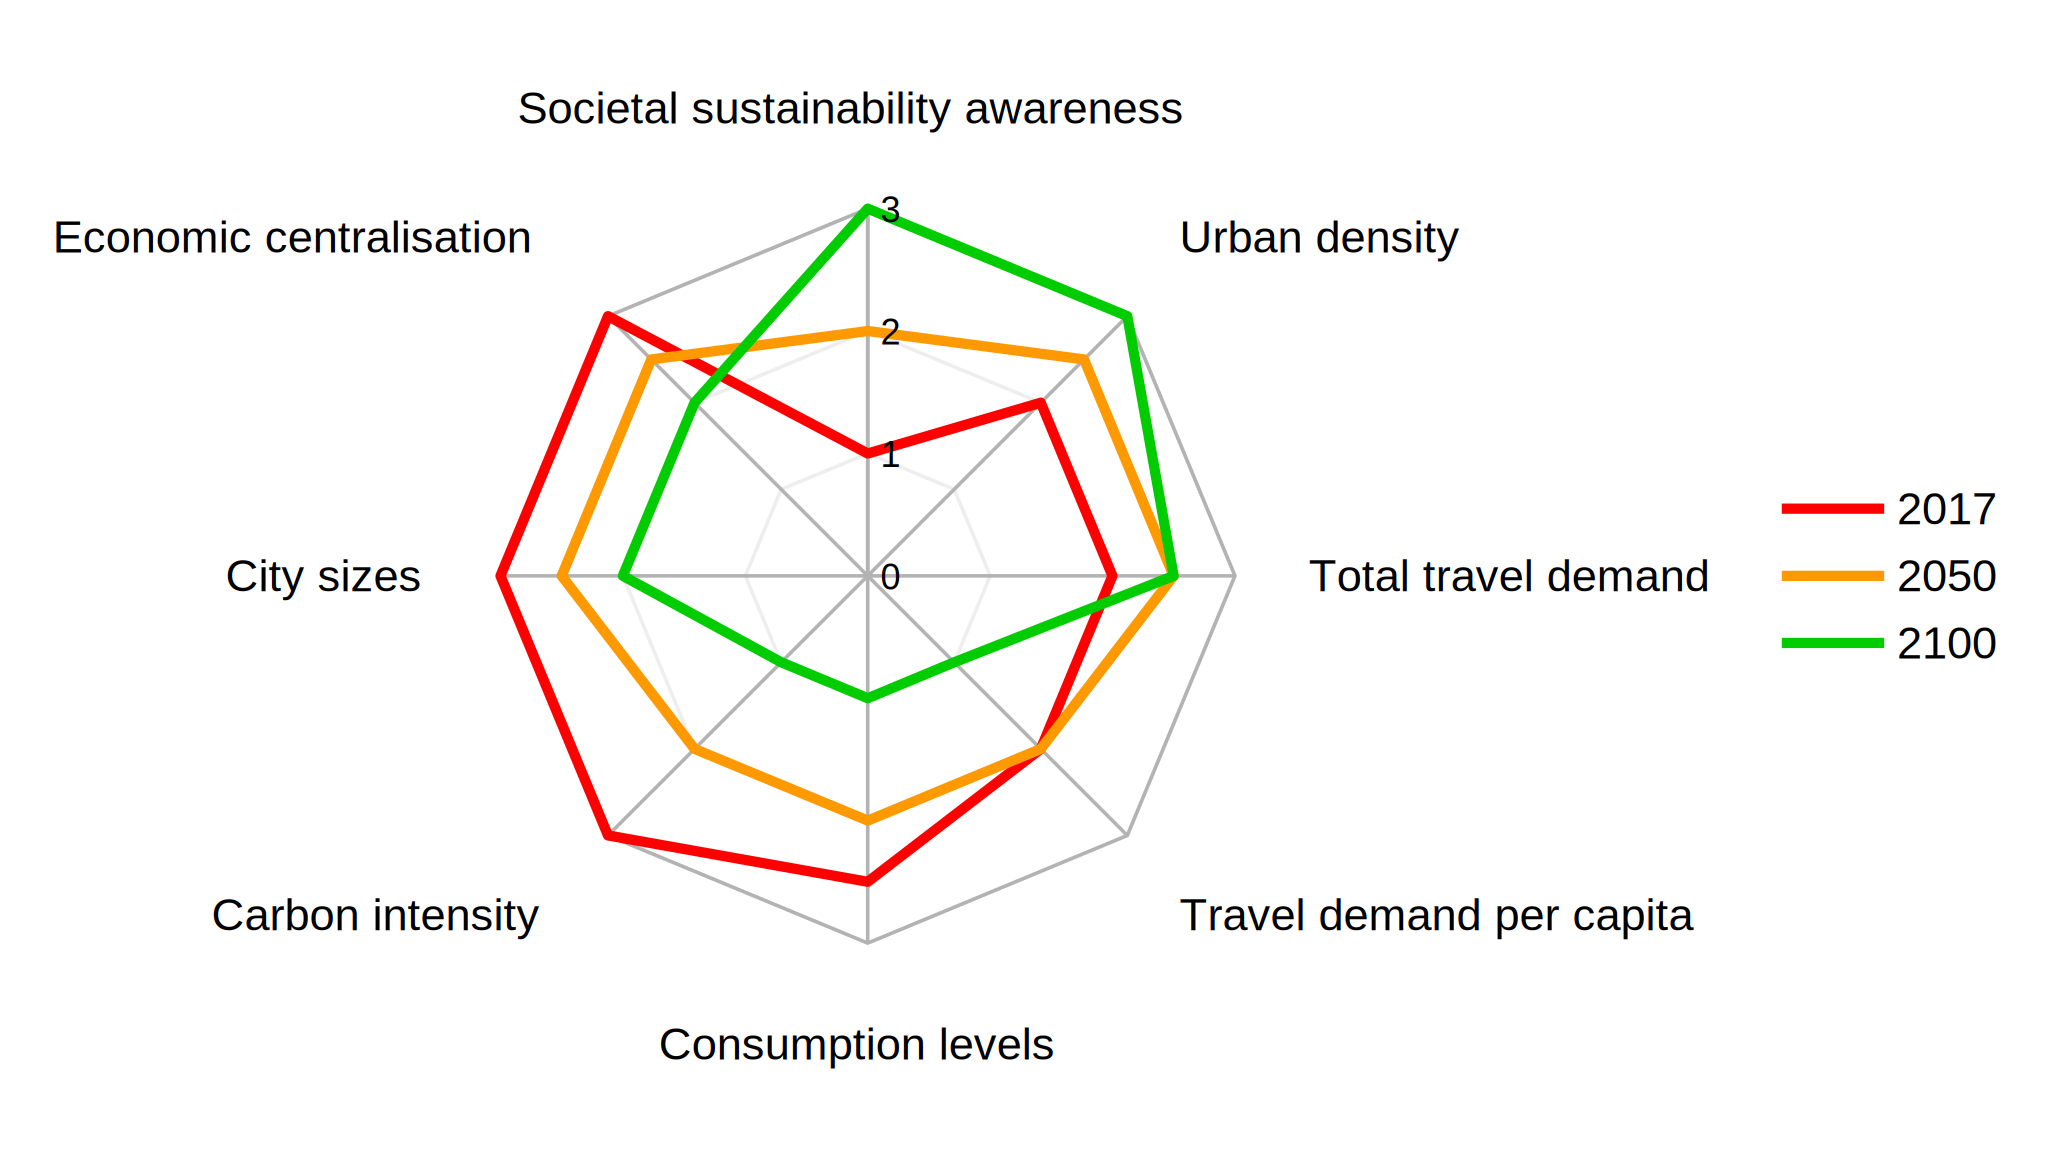
\includegraphics[width=0.8\textwidth]{figures/radar_development-scenario}
\caption[Shifts in development and land-use patterns in SSP1-MOB.]{Radar graph showing the shifts in development trends and land-use patterns found in SSP1 and SSP1-MOB for the years 2100, 2050 and 2017 (baseline). Values are given to the qualitative variables: 3 for high, 2 for medium and 1 for low.}
\label{fig:results:radar_development-scenario}
\end{figure}
%
\begin{figure}
		\centering
  \begin{subfigure}{0.8\textwidth}
    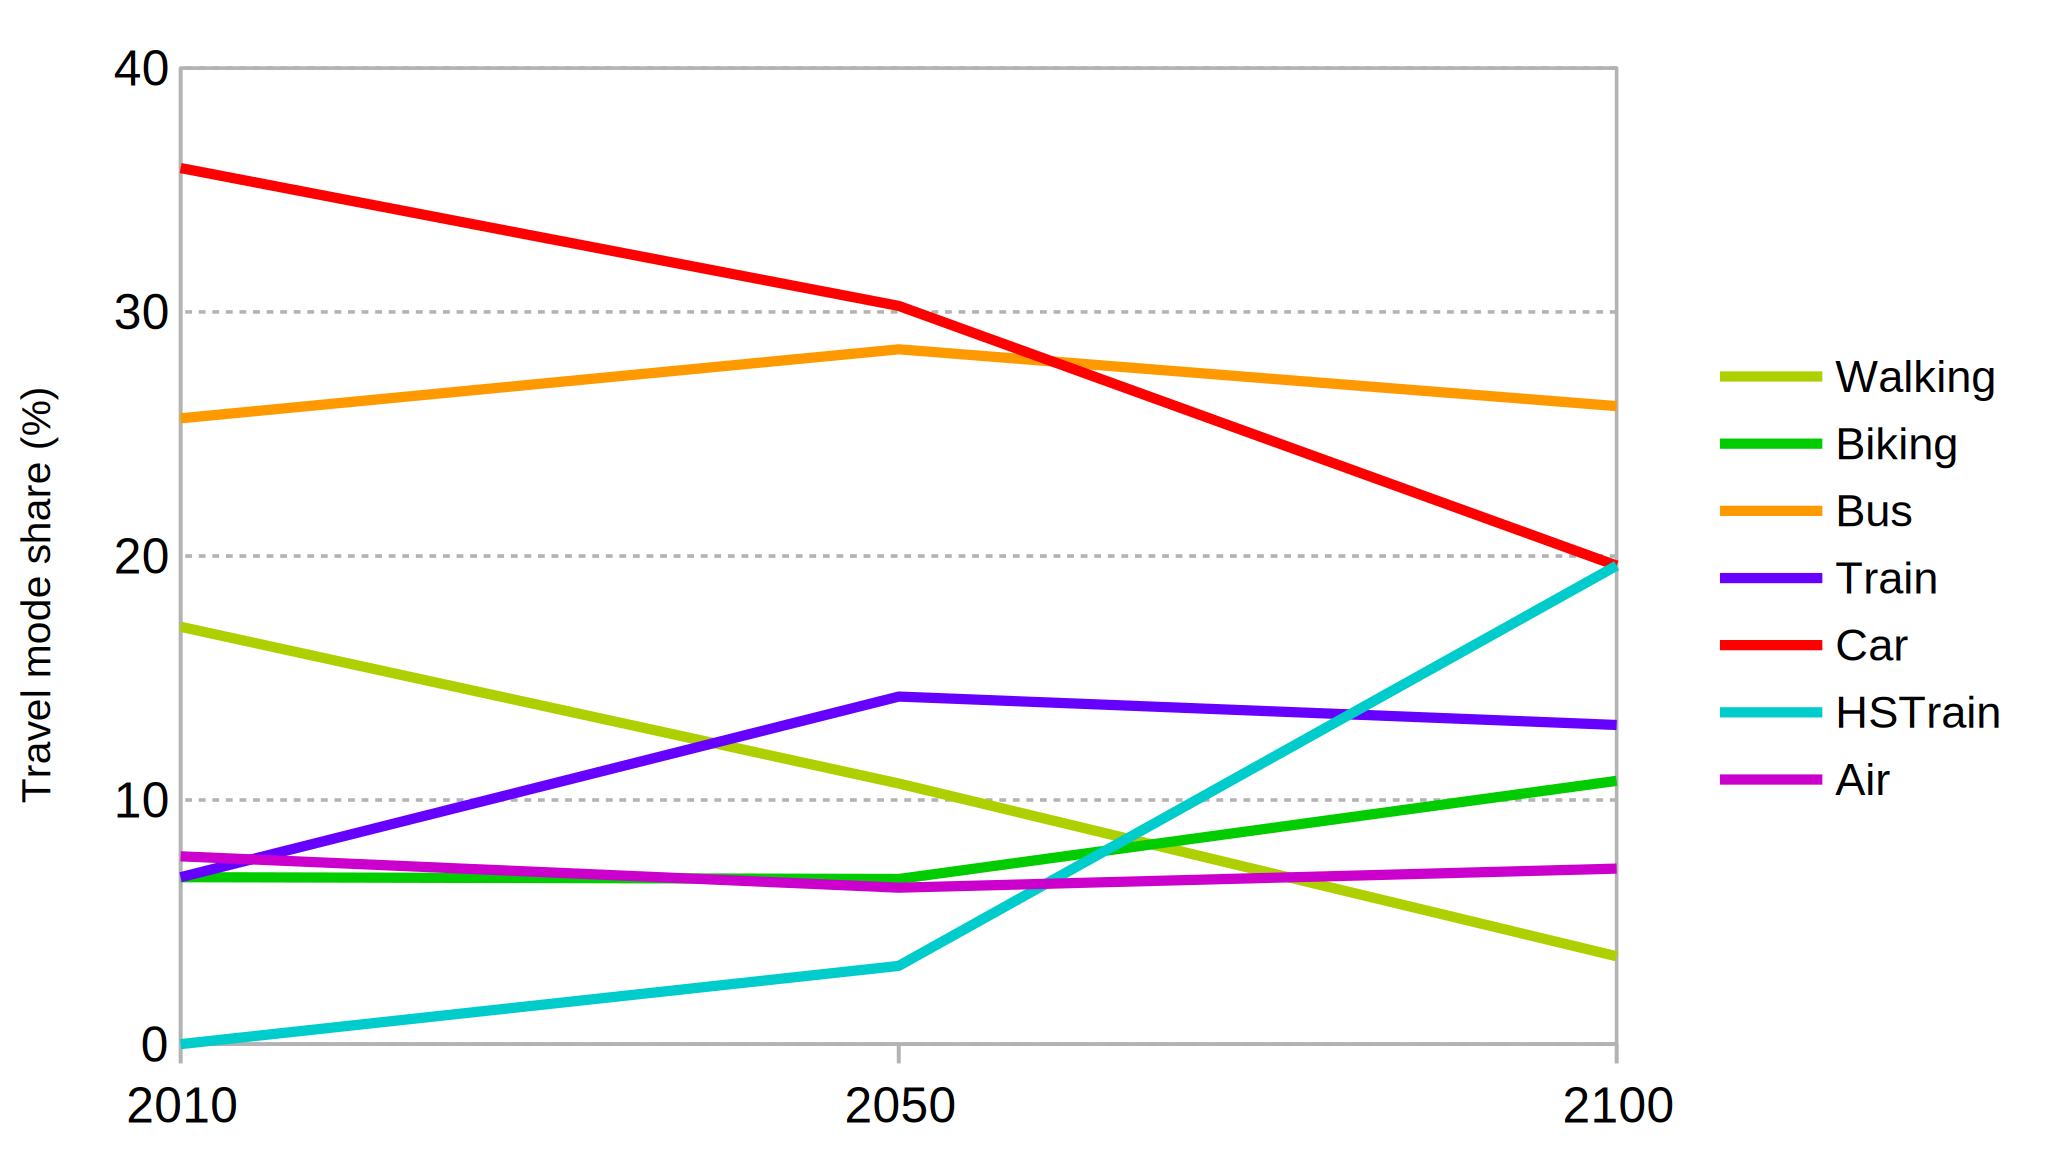
\includegraphics[width=\linewidth]{figures/line_travel-demand-shares.pdf}
    \caption{}
    \label{fig:results:line_travel-demand-shares}
  \end{subfigure}
  \begin{subfigure}{0.8\textwidth}
    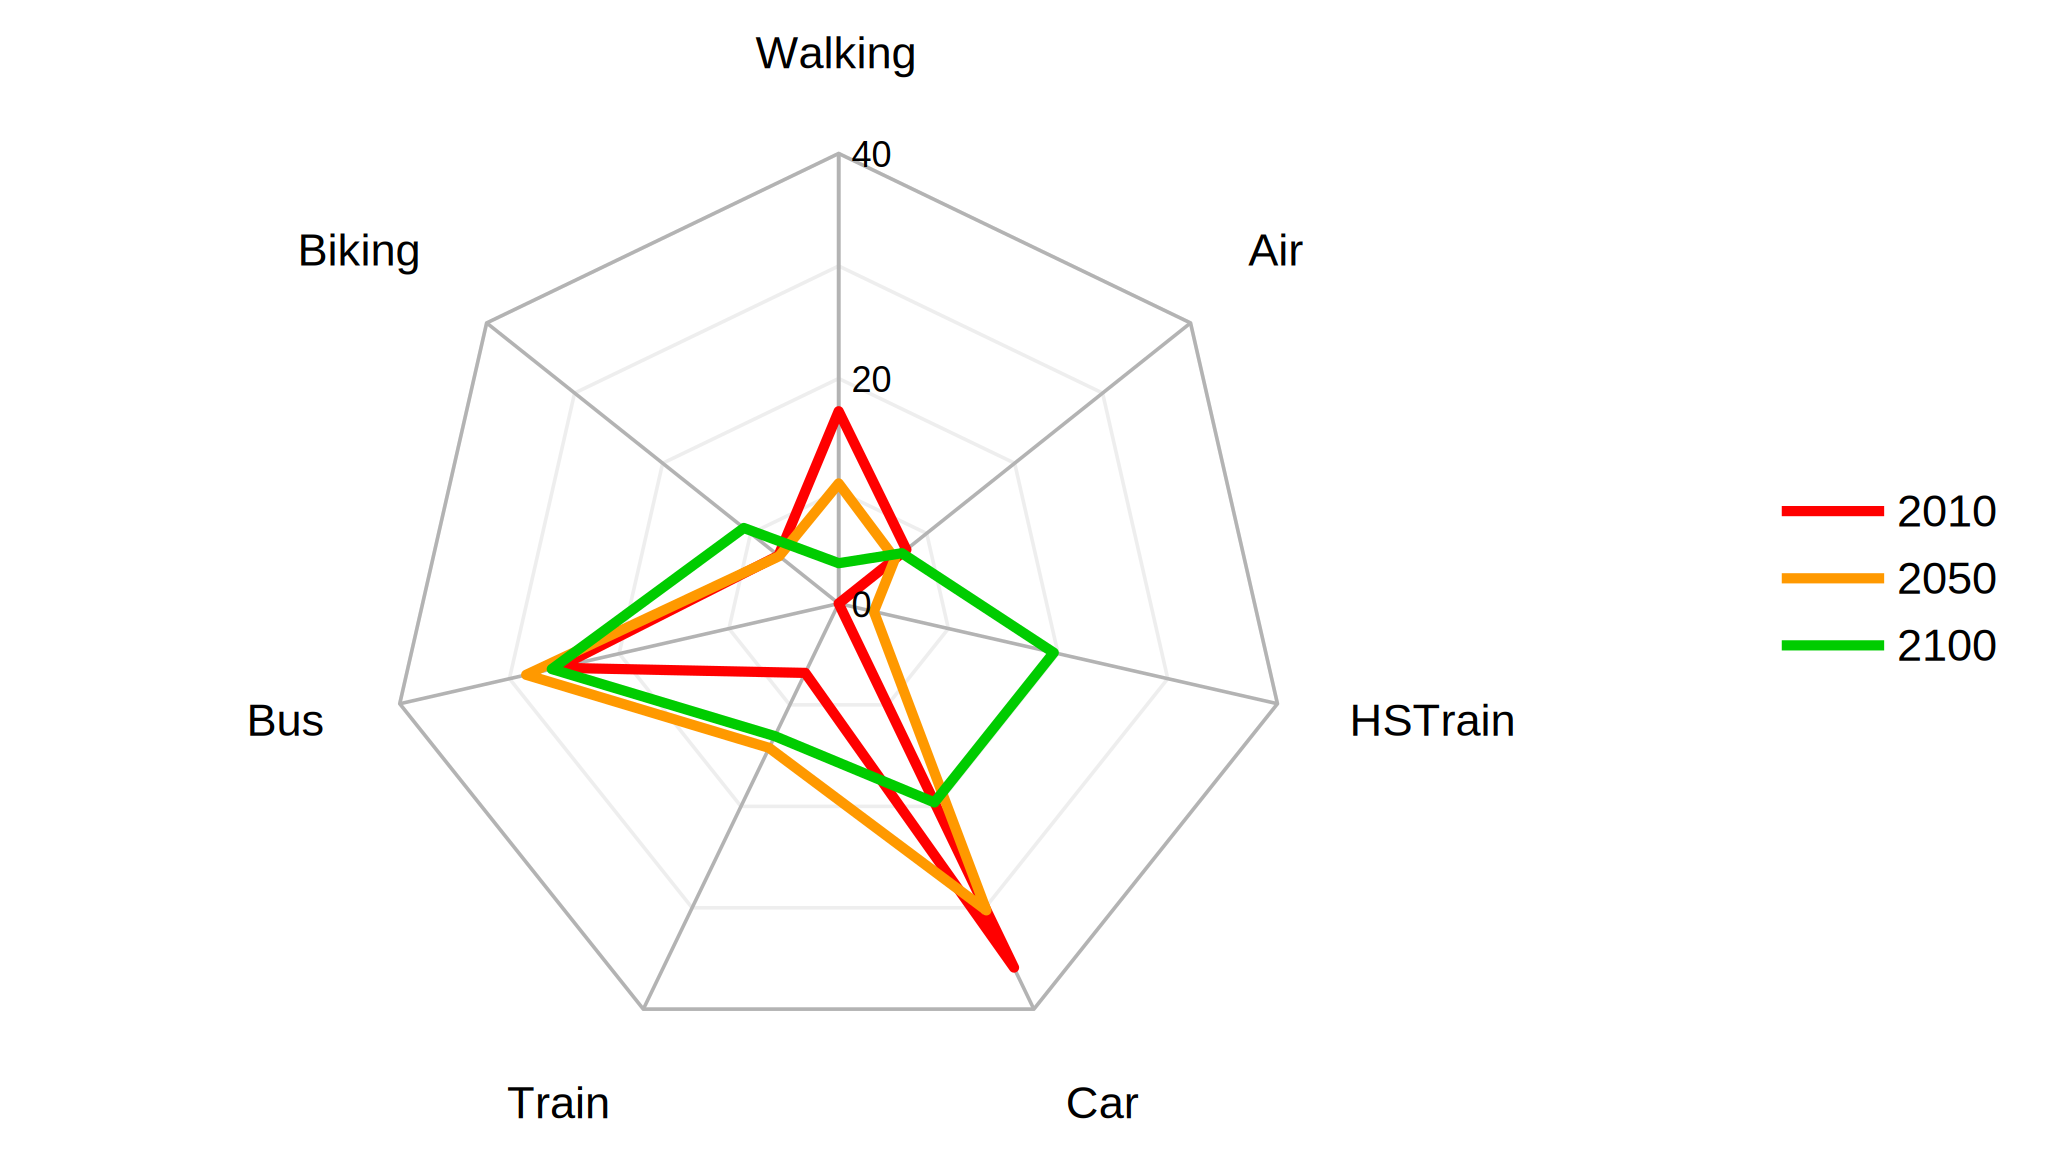
\includegraphics[width=\linewidth]{figures/radar_travel-demand-shares.pdf}
    \caption{}
    \label{fig:results:radar_travel-demand-shares}
  \end{subfigure}
  \caption[Evolution and comparison of travel demand shares in SSP1-MOB.]{Evolution (a) and comparison (b) of total travel demand per transport mode (shares), in percentages, across the SSP1-MOB futures and the 2017 baseline. Note: the demand shares are approximated from the figures provided by \textcite{vuuren2017_Energylanduse} in their quantitative appraisal of the SSP1 scenario.}
\end{figure}